\section{Từ bỏ Tích chập: Tại sao cần một Kiến trúc mới?}
\label{sec:moving_beyond_convolution}

Trong hơn một thập kỷ, các Mạng Nơ-ron Tích chập (CNN) đã ngự trị tối cao trong lĩnh vực thị giác máy tính. Từ chiến thắng mang tính lịch sử của AlexNet tại ImageNet 2012, các kiến trúc dựa trên tích chập đã không ngừng phát triển, ngày càng sâu hơn, hiệu quả hơn, và trở thành xương sống cho gần như mọi ứng dụng thị giác, từ các bài toán cơ bản như phân loại ảnh đến các hệ thống phức tạp trong xe tự hành hay chẩn đoán y tế.

Sức mạnh của CNN đến từ một \textbf{thiên kiến quy nạp (inductive bias)} mạnh mẽ và hợp lý: \textbf{tính cục bộ (locality)} và \textbf{bất biến với tịnh tiến (translation invariance)}. Giả định rằng các pixel lân cận có mối quan hệ mật thiết hơn các pixel ở xa, và một pattern (mẫu) có ý nghĩa ở một vị trí cũng sẽ có ý nghĩa ở vị trí khác, đã cho phép CNN học các biểu diễn hình ảnh một cách cực kỳ hiệu quả.

Tuy nhiên, khi quy mô dữ liệu ngày càng lớn và các bài toán trở nên phức tạp hơn, đòi hỏi sự hiểu biết ngữ nghĩa sâu sắc hơn và khả năng tích hợp với các dạng dữ liệu khác (như ngôn ngữ), chính thiên kiến quy nạp này bắt đầu bộc lộ những hạn chế cố hữu. Những "vết nứt" trong nền tảng của CNN đã dần xuất hiện, thôi thúc cộng đồng nghiên cứu tìm kiếm một mô thức kiến trúc mới, một kiến trúc có khả năng vượt qua những giới hạn của tính cục bộ.

\subsection{Hạn chế Cố hữu của Thiên kiến Tích chập}
\label{subsec:cnn_inductive_bias_limitations}
Mặc dù rất mạnh mẽ, các giả định nền tảng của CNN cũng chính là nguồn gốc của những hạn chế của nó trong việc mô hình hóa thế giới thị giác phức tạp.

\subsubsection{Trường thụ cảm Cục bộ và Hạn chế trong Lý luận Toàn cục}
\label{subsubsec:local_receptive_field}
Một lớp tích chập, bởi bản chất của nó, hoạt động như một bộ xử lý cục bộ. Mỗi nơ-ron trong một feature map chỉ "nhìn" thấy một vùng rất nhỏ của lớp trước đó, một vùng được gọi là \textbf{trường thụ cảm (receptive field)}. Mặc dù việc xếp chồng nhiều lớp lên nhau giúp mở rộng trường thụ cảm một cách từ từ, luồng thông tin vẫn mang tính cục bộ và phân cấp.

\begin{mdframed}[style=infobox]
	\textbf{Trực giác: Vấn đề của "Tầm nhìn Đường hầm"}
	
	Hãy tưởng tượng một nơ-ron ở lớp sâu của một mạng CNN đang cố gắng xác định xem một bức ảnh có chứa một con hươu cao cổ hay không. Nó có thể nhận được thông tin về một vùng có "kết cấu da hươu cao cổ" và một vùng khác có "hình dạng của một cái đầu có sừng". Tuy nhiên, hai vùng này có thể nằm ở hai đầu đối diện của bức ảnh. Để liên kết hai thông tin này, tín hiệu phải "di chuyển" qua rất nhiều lớp tích chập trung gian.
	
	Quá trình truyền thông tin gián tiếp này có thể làm nhiễu hoặc suy yếu tín hiệu. Mạng CNN gặp khó khăn trong việc thiết lập một mối liên kết trực tiếp và mạnh mẽ giữa các thành phần ngữ nghĩa xa nhau trong ảnh. Nó giống như việc cố gắng hiểu một bức tranh lớn bằng cách chỉ nhìn qua một loạt các ống nhòm nhỏ.
\end{mdframed}

Việc nắm bắt các \textbf{phụ thuộc tầm xa (long-range dependencies)} là cực kỳ quan trọng để hiểu được bối cảnh. Ví dụ, để phân biệt giữa một chiếc thuyền buồm và một cánh diều, việc nhận ra mối quan hệ giữa "cánh buồm" và "mặt nước" là điều then chốt. CNN gặp khó khăn trong việc thực hiện loại lý luận toàn cục này một cách hiệu quả.

\begin{center}
	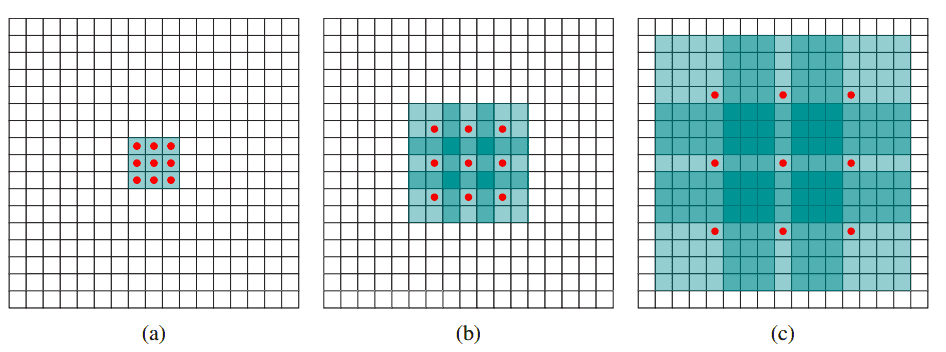
\includegraphics[width=0.9\textwidth]{images/cnn_receptive_field_growth.png}
	\captionof{figure}{Sự phát triển của trường thụ cảm trong một mạng CNN. Một nơ-ron ở các lớp sâu hơn (bên phải) có thể "nhìn" thấy một vùng lớn hơn của ảnh gốc, nhưng thông tin này là kết quả tổng hợp gián tiếp qua nhiều lớp trung gian.}
	\label{fig:cnn_receptive_field}
\end{center}
% Keyword gợi ý: cnn receptive field growth, convolutional neural network receptive field

\subsubsection{Trọng số Tĩnh và Thiếu khả năng Thích ứng với Nội dung}
\label{subsubsec:static_weights_content_agnostic}
Một đặc tính cơ bản khác của phép tích chập là các trọng số của kernel là \textbf{tĩnh (static)} và \textbf{độc lập với đầu vào (input-agnostic)}. Sau khi được huấn luyện, một kernel "phát hiện cạnh dọc" sẽ áp dụng chính xác cùng một bộ trọng số đó cho mọi vùng của mọi bức ảnh mà nó xử lý.

Điều này có nghĩa là CNN thiếu một cơ chế linh hoạt để "tập trung" vào các phần quan trọng của ảnh tùy thuộc vào nội dung. Nó xử lý một vùng trời xanh phẳng lặng với mức độ tính toán tương tự như một vùng chứa khuôn mặt người phức tạp. Khả năng phân bổ tài nguyên tính toán một cách linh hoạt, hay nói cách khác là khả năng "chú ý", không phải là một đặc tính tự nhiên của kiến trúc tích chập.

\subsection{Cảm hứng từ một Cuộc cách mạng Ngôn ngữ: Transformer}
\label{subsec:inspiration_from_nlp}
Trong khi lĩnh vực thị giác đang tìm cách vượt qua những giới hạn của tính cục bộ, một cuộc cách mạng đã âm thầm diễn ra trong lĩnh vực Xử lý Ngôn ngữ Tự nhiên (NLP). Năm 2017, bài báo có tựa đề \textbf{"Attention Is All You Need"} của Vaswani và các cộng sự đã giới thiệu kiến trúc \textbf{Transformer} \cite{Vaswani2017}.

Transformer đã từ bỏ hoàn toàn các kiến trúc tuần tự như Mạng Nơ-ron Hồi quy (RNN) và thay vào đó, chỉ dựa vào một cơ chế duy nhất: \textbf{Tự chú ý (Self-Attention)}.

\textbf{Nguyên lý của Self-Attention:} Thay vì xử lý từng từ trong một câu theo trình tự, cơ chế self-attention cho phép mỗi từ "nhìn" vào tất cả các từ khác trong câu cùng một lúc. Nó tính toán một "điểm số tương đồng" (attention score) giữa các từ, và sử dụng các điểm số này để tạo ra một biểu diễn mới cho mỗi từ, một biểu diễn đã được "làm giàu" bởi bối cảnh của toàn bộ câu. Một từ "bank" có thể "chú ý" nhiều hơn đến từ "river" hoặc "money" trong cùng một câu để xác định ý nghĩa chính xác của nó.

Những ưu điểm vượt trội của Transformer trong NLP là:
\begin{itemize}
	\item \textbf{Mô hình hóa quan hệ tầm xa xuất sắc:} Khoảng cách giữa các từ không còn là vấn đề.
	\item \textbf{Khả năng song song hóa cao:} Vì không có sự phụ thuộc tuần tự, việc tính toán có thể được thực hiện song song trên toàn bộ chuỗi, giúp huấn luyện hiệu quả trên các GPU.
	\item \textbf{Khả năng mở rộng (Scalability):} Kiến trúc này tỏ ra cực kỳ hiệu quả khi được mở rộng quy mô lên hàng tỷ, thậm chí hàng nghìn tỷ tham số.
\end{itemize}
Thành công phi thường của các mô hình như BERT và GPT đã chứng minh sức mạnh của triết lý dựa trên sự chú ý. Điều này đã làm dấy lên một câu hỏi tự nhiên: Liệu chúng ta có thể áp dụng cuộc cách mạng này cho thị giác?

\subsection{Tại sao Thị giác cần một Kiến trúc mới?}
\label{subsec:why_vision_needs_new_architecture}
Việc áp dụng triết lý của Transformer vào thị giác hứa hẹn sẽ giải quyết trực tiếp những hạn chế cố hữu của CNN.

\subsubsection{Lý luận Toàn cục (Global Reasoning)}
\label{subsubsec:global_reasoning_transformer}
Bằng cách coi một bức ảnh như một "chuỗi" các mảnh vá (patches), Transformer cho phép mỗi patch "chú ý" đến tất cả các patch khác. Điều này tạo ra một kênh giao tiếp trực tiếp giữa mọi vùng trong ảnh. Một patch ở góc trên bên trái có thể trực tiếp tính toán mối quan hệ của nó với một patch ở góc dưới bên phải, cho phép mô hình xây dựng một sự hiểu biết toàn cục về cấu trúc và bối cảnh của cảnh vật. Đây chính là lời giải cho bài toán phụ thuộc tầm xa.

\begin{center}
	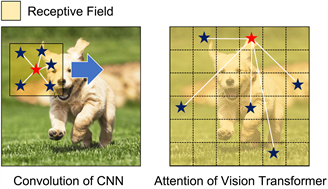
\includegraphics[width=1.0\textwidth]{images/cnn_vs_transformer_attention.png}
	\captionof{figure}{So sánh luồng thông tin. CNN (trái) xây dựng sự hiểu biết toàn cục một cách phân cấp và gián tiếp. Transformer (phải) cho phép mọi phần của đầu vào tương tác trực tiếp với nhau thông qua cơ chế self-attention.}
	\label{fig:cnn_vs_transformer_attention}
\end{center}
% Keyword gợi ý: cnn vs transformer attention, local vs global attention

\subsubsection{Kiến trúc Thống nhất cho Kỷ nguyên Đa phương thức}
\label{subsubsec:multimodality_foundation_models}
Một trong những lợi ích lớn nhất của Transformer là nó cung cấp một kiến trúc chung, linh hoạt có thể xử lý nhiều loại dữ liệu khác nhau. Dữ liệu, dù là văn bản, hình ảnh, hay âm thanh, đều có thể được "token hóa" thành một chuỗi các vector và được đưa vào cùng một kiến trúc Transformer.

Sự thống nhất này là nền tảng cho sự bùng nổ của các \textbf{mô hình đa phương thức (multimodal models)} và \textbf{mô hình nền tảng (foundation models)}:
\begin{itemize}
	\item Các mô hình như \textbf{CLIP} và \textbf{DALL-E} có thể học mối liên kết sâu sắc giữa hình ảnh và văn bản bằng cách xử lý cả hai trong cùng một không gian biểu diễn.
	\item Các Mô hình Ngôn ngữ Lớn Đa phương thức (Large Multimodal Models - LMMs) như \textbf{GPT-4o} và \textbf{Gemini} có thể "nhìn", "nghe", và "nói", xử lý một luồng thông tin liền mạch từ nhiều nguồn khác nhau.
\end{itemize}
CNN, với kiến trúc chuyên biệt cho dữ liệu dạng lưới 2D, không có được sự linh hoạt tự nhiên này.

\subsection{So sánh Triết lý Thiết kế: CNN vs. Transformer}
\label{subsec:philosophy_comparison}
Sự khác biệt giữa hai kiến trúc không chỉ nằm ở các phép toán, mà ở chính triết lý thiết kế nền tảng.

\begin{table}[h!]
	\centering
	\caption{So sánh triết lý thiết kế giữa CNN và Vision Transformer}
	\label{tab:cnn_vs_transformer_philosophy}
	\begin{tabularx}{\textwidth}{|l|X|X|}
		\hline
		\textbf{Đặc điểm} & \textbf{Mạng Nơ-ron Tích chập (CNN)} & \textbf{Vision Transformer (ViT)} \\
		\hline
		\textbf{Thiên kiến Quy nạp} & \textbf{Tính cục bộ} và \textbf{Bất biến tịnh tiến}. Giả định mạnh mẽ về cấu trúc dữ liệu. & \textbf{Tối thiểu}. Chỉ giả định ảnh có thể được chia thành các patch. Mọi mối quan hệ được học từ dữ liệu. \\
		\hline
		\textbf{Đơn vị Xử lý Cơ bản} & Phép tích chập trên các vùng pixel cục bộ. & Phép tự chú ý (Self-Attention) trên một tập hợp các vector patch. \\
		\hline
		\textbf{Luồng thông tin} & Phân cấp, từ cục bộ đến toàn cục một cách gián tiếp qua nhiều lớp. & Phẳng và toàn cục. Mọi patch có thể tương tác trực tiếp với nhau ngay từ lớp đầu tiên. \\
		\hline
		\textbf{Trọng số} & Tĩnh, độc lập với đầu vào (kernel được học và áp dụng cho mọi ảnh). & Động, phụ thuộc vào đầu vào (attention weights được tính toán lại cho mỗi ảnh). \\
		\hline
		\textbf{Nhu cầu Dữ liệu} & Hiệu quả hơn trên các bộ dữ liệu nhỏ và vừa do có thiên kiến mạnh. & Đói dữ liệu (data-hungry). Cần các bộ dữ liệu cực lớn hoặc pre-training quy mô lớn để học các quy luật thị giác từ đầu. \\
		\hline
		\textbf{Sự phù hợp Đa phương thức} & Hạn chế, cần các cơ chế kết hợp (fusion) đặc biệt. & Rất mạnh mẽ và tự nhiên, là nền tảng cho các mô hình đa phương thức. \\
		\hline
	\end{tabularx}
\end{table}

\subsection{Kết luận: Một sự Chuyển dịch Mô thức, không phải là sự Thay thế}
\label{subsec:paradigm_shift_conclusion}
Việc chuyển hướng sang các kiến trúc dựa trên Transformer không có nghĩa là CNN đã "lỗi thời" hay "vô dụng". CNN vẫn là một kiến trúc cực kỳ mạnh mẽ và hiệu quả, đặc biệt là trên các bộ dữ liệu có kích thước vừa phải và cho các ứng dụng không đòi hỏi sự hiểu biết ngữ nghĩa quá sâu sắc.

Tuy nhiên, sự trỗi dậy của Transformer đại diện cho một \textbf{sự chuyển dịch mô thức (paradigm shift)} quan trọng. Nó đánh dấu sự chuyển đổi từ một cách tiếp cận dựa trên các thiên kiến quy nạp mạnh mẽ, được lập trình cứng, sang một cách tiếp cận linh hoạt hơn, nơi các mối quan hệ được học hoàn toàn từ dữ liệu.

Transformer, với cơ chế self-attention mạnh mẽ, đã mở ra một kỷ nguyên mới của thị giác máy tính—một kỷ nguyên của lý luận toàn cục, của sự thống nhất giữa các dạng dữ liệu, và của các mô hình nền tảng quy mô lớn. Nó thay đổi cách chúng ta nghĩ về một bức ảnh: không còn chỉ là một ma trận pixel, mà là một tập hợp các "khái niệm" có mối quan hệ ngữ cảnh với nhau, sẵn sàng để được hiểu, diễn giải và tương tác.

\section*{Tài liệu tham khảo}
\begin{itemize}
	\item[1] Vaswani, A., Shazeer, N., Parmar, N., Uszkoreit, J., Jones, L., Gomez, A. N., ...\& Polosukhin, I. (2017). Attention is all you need. In \textit{Advances in neural information processing systems (NIPS)}. (Paper gốc giới thiệu kiến trúc Transformer).
	\item[2] Dosovitskiy, A., Beyer, L., Kolesnikov, A., Weissenborn, D., Zhai, X., Unterthiner, T., ...\& Houlsby, N. (2020). An image is worth 16x16 words: Transformers for image recognition at scale. \textit{arXiv preprint arXiv:2010.11929}. (Paper tiên phong áp dụng thành công kiến trúc Transformer cho bài toán phân loại ảnh - Vision Transformer).
	\item[3] He, K., Zhang, X., Ren, S.,\& Sun, J. (2016). Deep residual learning for image recognition. In \textit{Proceedings of the IEEE conference on computer vision and pattern recognition (CVPR)}. (Đại diện cho đỉnh cao của các kiến trúc CNN, làm nổi bật các hạn chế mà Transformer sau này nhắm đến để giải quyết).
	\item[4] Radford, A., Kim, J. W., Hallacy, C., Ramesh, A., Goh, G., Agarwal, S., ...\& Sutskever, I. (2021). Learning transferable visual models from natural language supervision. In \textit{International Conference on Machine Learning (ICML)}. (Một ví dụ điển hình về mô hình đa phương thức (CLIP) được xây dựng dựa trên triết lý của Transformer).
\end{itemize}